\documentclass{article}
\usepackage{graphicx} % Required for inserting images
\usepackage{subfig}
\usepackage{hyperref}
\usepackage{tcolorbox} 
\usepackage{subcaption} 
\usepackage{tikz}     % For drawing the border
\usepackage{float}
\usepackage{makecell}
\usepackage{booktabs}
\usepackage{multirow}
\usepackage{rotating}
\usepackage{tabularx}
\usepackage{xspace}
\usepackage{caption}
\usepackage{verbatim}

\renewcommand\tabularxcolumn[1]{m{#1}}% for vertical centering text in X column


%------- layout ------------
\oddsidemargin 0in
\topmargin 0in
\headheight 0in
\headsep 0 in
\textheight 8.7in
\textwidth 6.4in
%\hsize=6.7in
%\vsize=8.8in

\bibliographystyle{unsrt} 

 \graphicspath{{./plots/}} 

\begin{document}

% REAL WORLD DATASET DISTRIBUTIONS
\begin{figure}[!htbp]
\fbox
{
\begin{minipage}[t][0.98\textheight][t]{\textwidth}
\centering
    \vspace{20px}
    \begin{minipage}{0.95\linewidth}
    REAL-WORLD \\ DATASETS DISTRIBUTION
    \end{minipage}
    \vspace{20px}

   \begin{minipage}{0.49\linewidth}
        \begin{figure}[H]
        \includegraphics[width=\linewidth]{plots/dataset_distribution/books_200M_uint32}
        \caption{Amzn uint32}
        \end{figure}
    \end{minipage}
    \begin{minipage}{0.49\linewidth}
        \begin{figure}[H]
            \includegraphics[width=\linewidth]{plots/dataset_distribution/companynet_uint32}
            \caption{CompanyNet}
        \end{figure}
    \end{minipage}

    \vfill

    \begin{minipage}{0.49\linewidth}
        \begin{figure}[H]
        \includegraphics[width=\linewidth]{plots/dataset_distribution/friendster_50M_uint32}
        \caption{Friendster}
        \end{figure}
    \end{minipage}
    \begin{minipage}{0.49\linewidth}
        \begin{figure}[H]
            \includegraphics[width=\linewidth]{plots/dataset_distribution/wiki_ts_200M_uint32}
            \caption{Wiki uint32}
        \end{figure}
    \end{minipage}
    
    \vfill
    \centering
    \begin{minipage}{\linewidth}
    Real-world datasets - distribution. The $x$ axis reports the indexes (positions) in the vector to store, while the $y$ axis reports the corresponding values.
    \end{minipage}
    \vspace{10px}
\end{minipage}
}
\end{figure}

% distribution SYNTH
\begin{figure}[!htbp]
\fbox
{
\begin{minipage}[t][0.98\textheight][t]{\textwidth}
\centering
    \vspace{20px}
    \begin{minipage}{0.95\linewidth}
    SYNTHETIC DATASETS \\ DISTRIBUTION
    \end{minipage}
    \vspace{20px}

   \begin{minipage}{0.49\linewidth}
        \begin{figure}[H]
        \includegraphics[width=\linewidth]{plots/dataset_distribution/normal_uint32}
        \caption{Normal}
        \end{figure}
    \end{minipage}
    \begin{minipage}{0.49\linewidth}
        \begin{figure}[H]
            \includegraphics[width=\linewidth]{plots/dataset_distribution/lognormal_uint32}
            \caption{Lognormal}
        \end{figure}
    \end{minipage}

    \vfill
    
    \begin{minipage}{0.49\linewidth}
        \begin{figure}[H]
        \includegraphics[width=\linewidth]{plots/dataset_distribution/exponential_uint32}
        \caption{Exponential}
        \end{figure}
    \end{minipage}
    \begin{minipage}{0.49\linewidth}
        \begin{figure}[H]
            \includegraphics[width=\linewidth]{plots/dataset_distribution/zipf_uint32}
            \caption{Zipf}
        \end{figure}
    \end{minipage}

    \vfill
    \centering
    \begin{minipage}{\linewidth}
        Synthetic dataset - distribution. The $x$ axis reports the indexes (positions) in the vector to store, while the $y$ axis reports the corresponding values.
    \end{minipage}
    \vspace{10px}
\end{minipage}
}
\end{figure}

% distribution uint64
\begin{figure}[!htbp]
\fbox
{
\begin{minipage}[t][0.98\textheight][t]{\textwidth}
\centering
    \vspace{20px}
    \begin{minipage}{0.95\linewidth}
    64-BIT DATASETS \\ DISTRIBUTION
    \end{minipage}
    \vspace{20px}

   \begin{minipage}{0.49\linewidth}
        \begin{figure}[H]
        \includegraphics[width=\linewidth]{plots/dataset_distribution/books_800M_uint64}
        \caption{Amzn uint64}
        \end{figure}
    \end{minipage}
    \begin{minipage}{0.49\linewidth}
        \begin{figure}[H]
            \includegraphics[width=\linewidth]{plots/dataset_distribution/fb_200M_uint64}
            \caption{Facebook uint64}
        \end{figure}
    \end{minipage}

    \vfill
    
    \begin{minipage}{0.49\linewidth}
        \begin{figure}[H]
        \includegraphics[width=\linewidth]{plots/dataset_distribution/osm_cellids_800M_uint64}
        \caption{OSM Cellids uint64}
        \end{figure}
    \end{minipage}
    \begin{minipage}{0.49\linewidth}
        \begin{figure}[H]
            \includegraphics[width=\linewidth]{plots/dataset_distribution/wiki_ts_200M_uint64}
            \caption{Wiki uint64}
        \end{figure}
    \end{minipage}

    \vfill
    \centering
    \begin{minipage}{\linewidth}
        64-bits datasets - dataset distributions. The $x$ axis reports the indexes (positions) in the vector to store, while the $y$ axis reports the corresponding values.
    \end{minipage}
    \vspace{10px}
\end{minipage}
}
\end{figure}

% BUILDTIME REAL WORLD
\begin{figure}[!htbp]
\fbox
{
\begin{minipage}[t][0.98\textheight][t]{\textwidth}
\centering
    \begin{minipage}{0.2\linewidth}
    \footnotesize{BUILD TIME ON \\ REAL-WORLD DATASETS}
    \end{minipage}
   \begin{minipage}{0.75\linewidth}
        \begin{figure}[H]
        \includegraphics[width=\linewidth]{plots/legends/all.png}
        \end{figure}
    \end{minipage}
    \vspace*{-10px}
    
    \begin{minipage}{0.03\linewidth}
    \begin{sideways}\small COMPANYNET\end{sideways}
    \end{minipage}
    \begin{minipage}{0.39\linewidth}
        \begin{figure}[H]
        \includegraphics[width=\linewidth]{plots/buildtime/companynet_uint32.png}
        \end{figure}
    \end{minipage}
    \begin{minipage}{0.39\linewidth}
        \begin{figure}[H]
            \includegraphics[width=\linewidth]{plots/buildtime/zoom/companynet_uint32.png}
        \end{figure}
    \end{minipage}
\vspace*{-0.55cm}

\begin{minipage}{0.03\linewidth}
    \begin{sideways}\small FRIENDSTER\end{sideways}
    \end{minipage}
    \begin{minipage}{0.39\linewidth}
        \begin{figure}[H]
        \includegraphics[width=\linewidth]{plots/buildtime/friendster_50M_uint32.png}
        \end{figure}
    \end{minipage}
    \begin{minipage}{0.39\linewidth}
        \begin{figure}[H]
            \includegraphics[width=\linewidth]{plots/buildtime/zoom/friendster_50M_uint32.png}
        \end{figure}
    \end{minipage}
\vspace*{-0.55cm}

    \begin{minipage}{0.03\linewidth}
    \begin{sideways}\small AMZN\end{sideways}
    \end{minipage}
   \begin{minipage}{0.39\linewidth}
        \begin{figure}[H]
        \includegraphics[width=\linewidth]{plots/buildtime/books_200M_uint32.png}
        \end{figure}
    \end{minipage}
    \begin{minipage}{0.39\linewidth}
        \begin{figure}[H]
            \includegraphics[width=\linewidth]{plots/buildtime/zoom/books_200M_uint32.png}
        \end{figure}
    \end{minipage}
\vspace*{-0.55cm}

    \begin{minipage}{0.03\linewidth}
    \begin{sideways}\small WIKI\end{sideways}
    \end{minipage}
    \begin{minipage}{0.39\linewidth}
        \begin{figure}[H]
        \includegraphics[width=\linewidth]{plots/buildtime/wiki_ts_200M_uint32.png}
        \end{figure}
    \end{minipage}
    \begin{minipage}{0.39\linewidth}
        \begin{figure}[H]
            \includegraphics[width=\linewidth]{plots/buildtime/zoom/wiki_ts_200M_uint32.png}
        \end{figure}
    \end{minipage}

    \vfill
    \centering
    \begin{minipage}{\linewidth}
        The plots above report the time required to build the data structures (indexes) on the real-world datasets. On the left, the dataset's name is shown; in the middle, the complete plot with all the times expressed in milliseconds; and on the right, the same plot but excluding the ones with excessive build times (those that are over double the average of all build times of all indexes).
    \end{minipage}
    \vspace{10px}
\end{minipage}
}
\caption{Build time on real-world datasets}
\end{figure}

% BUILDTIME SYNTH
\begin{figure}[!htbp]
\fbox
{
\begin{minipage}[t][0.98\textheight][t]{\textwidth}
\centering
    \begin{minipage}{0.2\linewidth}
    \footnotesize{BUILD TIME ON \\ SYNTHETIC DATASETS}
    \end{minipage}
   \begin{minipage}{0.75\linewidth}
        \begin{figure}[H]
        \includegraphics[width=\linewidth]{plots/legends/all.png}
        \end{figure}
    \end{minipage}
    \vspace*{-10px}
    
    \begin{minipage}{0.03\linewidth}
    \begin{sideways}\small NORMAL\end{sideways}
    \end{minipage}
    \begin{minipage}{0.39\linewidth}
        \begin{figure}[H]
        \includegraphics[width=\linewidth]{plots/buildtime/normal_uint32.png}
        \end{figure}
    \end{minipage}
    \begin{minipage}{0.39\linewidth}
        \begin{figure}[H]
            \includegraphics[width=\linewidth]{plots/buildtime/zoom/normal_uint32.png}
        \end{figure}
    \end{minipage}
\vspace*{-0.55cm}

\begin{minipage}{0.03\linewidth}
    \begin{sideways}\small LOGNORMAL\end{sideways}
    \end{minipage}
    \begin{minipage}{0.39\linewidth}
        \begin{figure}[H]
        \includegraphics[width=\linewidth]{plots/buildtime/lognormal_uint32.png}
        \end{figure}
    \end{minipage}
    \begin{minipage}{0.39\linewidth}
        \begin{figure}[H]
            \includegraphics[width=\linewidth]{plots/buildtime/zoom/lognormal_uint32.png}
        \end{figure}
    \end{minipage}
\vspace*{-0.55cm}

    \begin{minipage}{0.03\linewidth}
    \begin{sideways}\small EXPONENTIAL\end{sideways}
    \end{minipage}
   \begin{minipage}{0.39\linewidth}
        \begin{figure}[H]
        \includegraphics[width=\linewidth]{plots/buildtime/exponential_uint32.png}
        \end{figure}
    \end{minipage}
    \begin{minipage}{0.39\linewidth}
        \begin{figure}[H]
            \includegraphics[width=\linewidth]{plots/buildtime/zoom/exponential_uint32.png}
        \end{figure}
    \end{minipage}
\vspace*{-0.55cm}

    \begin{minipage}{0.03\linewidth}
    \begin{sideways}\small ZIPF\end{sideways}
    \end{minipage}
    \begin{minipage}{0.39\linewidth}
        \begin{figure}[H]
        \includegraphics[width=\linewidth]{plots/buildtime/zipf_uint32.png}
        \end{figure}
    \end{minipage}
    \begin{minipage}{0.39\linewidth}
        \begin{figure}[H]
            \includegraphics[width=\linewidth]{plots/buildtime/zoom/zipf_uint32.png}
        \end{figure}
    \end{minipage}

    \vfill
    \centering
    \begin{minipage}{\linewidth}
The plots above report the time required to build the data structures (indexes) on the synthetic datasets. On the left, the dataset's name is shown; in the middle, the complete plot with all the times expressed in milliseconds; and on the right, the same plot but excluding the ones with excessive build times (those that are over double the average of all build times of all indexes).
    \end{minipage}
    \vspace{10px}
\end{minipage}
}
\caption{Build time on synthetic datasets}
\end{figure}

% BUILDTIME uint64
\begin{figure}[!htbp]
\fbox
{
\begin{minipage}[t][0.98\textheight][t]{\textwidth}
\centering
    \begin{minipage}{0.2\linewidth}
    \footnotesize{BUILD TIME ON  \\ 64-BIT DATASETS}
    \end{minipage}
   \begin{minipage}{0.75\linewidth}
        \begin{figure}[H]
        \includegraphics[width=\linewidth]{plots/legends/all.png}
        \end{figure}
    \end{minipage}
    \vspace*{-10px}
    
    \begin{minipage}{0.03\linewidth}
    \begin{sideways}\small AMZN64\end{sideways}
    \end{minipage}
    \begin{minipage}{0.39\linewidth}
        \begin{figure}[H]
        \includegraphics[width=\linewidth]{plots/buildtime/books_800M_uint64.png}
        \end{figure}
    \end{minipage}
    \begin{minipage}{0.39\linewidth}
        \begin{figure}[H]
            \includegraphics[width=\linewidth]{plots/buildtime/zoom/books_800M_uint64.png}
        \end{figure}
    \end{minipage}
\vspace*{-0.55cm}

\begin{minipage}{0.03\linewidth}
    \begin{sideways}\small FACEBOOK64\end{sideways}
    \end{minipage}
    \begin{minipage}{0.39\linewidth}
        \begin{figure}[H]
        \includegraphics[width=\linewidth]{plots/buildtime/fb_200M_uint64.png}
        \end{figure}
    \end{minipage}
    \begin{minipage}{0.39\linewidth}
        \begin{figure}[H]
            \includegraphics[width=\linewidth]{plots/buildtime/zoom/fb_200M_uint64.png}
        \end{figure}
    \end{minipage}
\vspace*{-0.55cm}

    \begin{minipage}{0.03\linewidth}
    \begin{sideways}\small OSM CELLIDS 64\end{sideways}
    \end{minipage}
   \begin{minipage}{0.39\linewidth}
        \begin{figure}[H]
        \includegraphics[width=\linewidth]{plots/buildtime/osm_cellids_800M_uint64.png}
        \end{figure}
    \end{minipage}
    \begin{minipage}{0.39\linewidth}
        \begin{figure}[H]
            \includegraphics[width=\linewidth]{plots/buildtime/zoom/osm_cellids_800M_uint64.png}
        \end{figure}
    \end{minipage}
\vspace*{-0.55cm}

    \begin{minipage}{0.03\linewidth}
    \begin{sideways}\small WIKI 64\end{sideways}
    \end{minipage}
    \begin{minipage}{0.4\linewidth}
        \begin{figure}[H]
        \includegraphics[width=\linewidth]{plots/buildtime/wiki_ts_200M_uint64.png}
        \end{figure}
    \end{minipage}
    \begin{minipage}{0.39\linewidth}
        \begin{figure}[H]
            \includegraphics[width=\linewidth]{plots/buildtime/zoom/wiki_ts_200M_uint64.png}
        \end{figure}
    \end{minipage}

    \vfill
    \centering
    \begin{minipage}{\linewidth}
        The plots above report the time required to build the data structures (indexes) on the 64-bit datasets. On the left, the dataset's name is shown; in the middle, the complete plot with all the times expressed in milliseconds; and on the right, the same plot but excluding the ones with excessive build times (those that are over double the average of all build times of all indexes).
    \end{minipage}
    \vspace{10px}
\end{minipage}
}
\caption{Build time on 64-bit datasets}
\end{figure}

% INDEX LOOKUP REAL WORLD
\begin{figure}[!htbp]
\fbox
{
\begin{minipage}[t][0.98\textheight][t]{\textwidth}
\centering 
    \begin{minipage}{0.23\linewidth}
    \footnotesize{TRADITIONAL/LEARNED INDEXES::\\SEARCH TIME ON \\ REAL DATASET}
    \end{minipage}
   \begin{minipage}{0.7\linewidth}
        \begin{figure}[H]
        \includegraphics[width=\linewidth]{plots/legends/index.png}
        \end{figure}
    \end{minipage}
    \vspace*{-10px}

    \begin{minipage}{0.05\linewidth}
    \begin{sideways}\small COMPANYNET\end{sideways}
    \end{minipage}
    \begin{minipage}{0.32\linewidth}
        \begin{figure}[H]
        \includegraphics[width=\linewidth]{plots/index/companynet_uint32.png}
        \end{figure}
    \end{minipage}
    \begin{minipage}{0.32\linewidth}
        \begin{figure}[H]
            \includegraphics[width=\linewidth]{plots/index/space/companynet_uint32.png}
        \end{figure}
    \end{minipage}
    \vspace*{-16px}

    \begin{minipage}{0.05\linewidth}
    \begin{sideways}\small FRIENDSTER\end{sideways}
    \end{minipage}
    \begin{minipage}{0.32\linewidth}
        \begin{figure}[H]
        \includegraphics[width=\linewidth]{plots/index/friendster_50M_uint32.png}
        \end{figure}
    \end{minipage}
    \begin{minipage}{0.32\linewidth}
        \begin{figure}[H]
            \includegraphics[width=\linewidth]{plots/index/space/friendster_50M_uint32.png}
        \end{figure}
    \end{minipage}
    \vspace*{-16px}

    \begin{minipage}{0.05\linewidth}
    \begin{sideways}\small AMZN\end{sideways}
    \end{minipage}
    \begin{minipage}{0.32\linewidth}
        \begin{figure}[H]
        \includegraphics[width=\linewidth]{plots/index/books_200M_uint32.png}
        \end{figure}
    \end{minipage}
    \begin{minipage}{0.32\linewidth}
        \begin{figure}[H]
            \includegraphics[width=\linewidth]{plots/index/space/books_200M_uint32.png}
        \end{figure}
    \end{minipage}
    \vspace*{-16px}

    \begin{minipage}{0.05\linewidth}
    \begin{sideways}\small WIKI\end{sideways}
    \end{minipage}
    \begin{minipage}{0.32\linewidth}
        \begin{figure}[H]
        \includegraphics[width=\linewidth]{plots/index/wiki_ts_200M_uint32.png}
        \end{figure}
    \end{minipage}
    \begin{minipage}{0.32\linewidth}
        \begin{figure}[H]
            \includegraphics[width=\linewidth]{plots/index/space/wiki_ts_200M_uint32.png}
        \end{figure}
    \end{minipage}

    \vfill
    
    \centering
    \begin{minipage}{\linewidth}
        The performances of traditional and learned indexes on real-world datasets are represented in two plots. The leftmost plot shows the time of search (in ns) on each index; while the right plot shows the space occupied by each index in MBs (without considering the space occupied by the data to be stored). The left plot shows two bars for each data structure. The left/right one shows the average time to search for an existing/missing item in the collection.
    \end{minipage}
    \vspace{10px}
\end{minipage}
}
\caption{Average time for pointwise queries on traditional and learned indexes, built on real-world datasets.}
\end{figure}

% INDEX LOOKUP SYNTH
\begin{figure}[!htbp]
\fbox
{
\begin{minipage}[t][0.98\textheight][t]{\textwidth}
\centering
    \begin{minipage}{0.23\linewidth}
    \footnotesize{TRADITIONAL/LEARNED INDEXES::\\SEARCH TIME ON \\ SYNTHETIC DATASET}
    \end{minipage}
   \begin{minipage}{0.7\linewidth}
        \begin{figure}[H]
        \includegraphics[width=\linewidth]{plots/legends/index.png}
        \end{figure}
    \end{minipage}
    \vspace*{-10px}

    \begin{minipage}{0.05\linewidth}
    \begin{sideways}\small NORMAL\end{sideways}
    \end{minipage}
    \begin{minipage}{0.32\linewidth}
        \begin{figure}[H]
        \includegraphics[width=\linewidth]{plots/index/normal_uint32.png}
        \end{figure}
    \end{minipage}
    \begin{minipage}{0.32\linewidth}
        \begin{figure}[H]
            \includegraphics[width=\linewidth]{plots/index/space/normal_uint32.png}
        \end{figure}
    \end{minipage}
    \vspace*{-16px}

    \begin{minipage}{0.05\linewidth}
    \begin{sideways}\small LOGNORMAL\end{sideways}
    \end{minipage}
    \begin{minipage}{0.32\linewidth}
        \begin{figure}[H]
        \includegraphics[width=\linewidth]{plots/index/lognormal_uint32.png}
        \end{figure}
    \end{minipage}
    \begin{minipage}{0.32\linewidth}
        \begin{figure}[H]
            \includegraphics[width=\linewidth]{plots/index/space/lognormal_uint32.png}
        \end{figure}
    \end{minipage}
    \vspace*{-16px}

    \begin{minipage}{0.05\linewidth}
    \begin{sideways}\small EXPONENTIAL\end{sideways}
    \end{minipage}
    \begin{minipage}{0.32\linewidth}
        \begin{figure}[H]
        \includegraphics[width=\linewidth]{plots/index/exponential_uint32.png}
        \end{figure}
    \end{minipage}
    \begin{minipage}{0.32\linewidth}
        \begin{figure}[H]
            \includegraphics[width=\linewidth]{plots/index/space/exponential_uint32.png}
        \end{figure}
    \end{minipage}
    \vspace*{-16px}

    \begin{minipage}{0.05\linewidth}
    \begin{sideways}\small ZIPF\end{sideways}
    \end{minipage}
    \begin{minipage}{0.32\linewidth}
        \begin{figure}[H]
        \includegraphics[width=\linewidth]{plots/index/zipf_uint32.png}
        \end{figure}
    \end{minipage}
    \begin{minipage}{0.32\linewidth}
        \begin{figure}[H]
            \includegraphics[width=\linewidth]{plots/index/space/zipf_uint32.png}
        \end{figure}
    \end{minipage}
    \vfill
    
    \centering
    \begin{minipage}{\linewidth}
        The performance of traditional and learned indexes on synthetic datasets are represented in two plots. The leftmost plot shows the time of search (in ns) on each index; while the right plot shows the space occupied by each index in MBs (without considering the space occupied by the data to be stored). The left plot shows two bars for each data structure. The left/right one shows the average time to search for an existing/missing item in the collection.
    \end{minipage}
    \vspace{10px}
\end{minipage}
}
\caption{Average time for pointwise queries on traditional and learned indexes, built on synthetic datasets.}
\end{figure}

% INDEX LOOKUP uint64
\begin{figure}[!htbp]
\fbox
{
\begin{minipage}[t][0.98\textheight][t]{\textwidth}
\centering
    \begin{minipage}{0.23\linewidth}
    \footnotesize{TRADITIONAL/LEARNED INDEXES::\\SEARCH TIME ON \\ 64-BIT DATASET}
    \end{minipage}
   \begin{minipage}{0.7\linewidth}
        \begin{figure}[H]
        \includegraphics[width=\linewidth]{plots/legends/index.png}
        \end{figure}
    \end{minipage}
    \vspace*{-10px}

    \begin{minipage}{0.05\linewidth}
    \begin{sideways}\small AMZN 64 \end{sideways}
    \end{minipage}
    \begin{minipage}{0.32\linewidth}
        \begin{figure}[H]
        \includegraphics[width=\linewidth]{plots/index/books_800M_uint64.png}
        \end{figure}
    \end{minipage}
    \begin{minipage}{0.32\linewidth}
        \begin{figure}[H]
            \includegraphics[width=\linewidth]{plots/index/space/books_800M_uint64.png}
        \end{figure}
    \end{minipage}
    \vspace*{-15px}

    \begin{minipage}{0.05\linewidth}
    \begin{sideways}\small FACEBOOK 64\end{sideways}
    \end{minipage}
    \begin{minipage}{0.32\linewidth}
        \begin{figure}[H]
        \includegraphics[width=\linewidth]{plots/index/fb_200M_uint64.png}
        \end{figure}
    \end{minipage}
    \begin{minipage}{0.32\linewidth}
        \begin{figure}[H]
            \includegraphics[width=\linewidth]{plots/index/space/fb_200M_uint64.png}
        \end{figure}
    \end{minipage}
    \vspace*{-15px}

    \begin{minipage}{0.05\linewidth}
    \begin{sideways}\small OSM CELLIDS 64\end{sideways}
    \end{minipage}
    \begin{minipage}{0.32\linewidth}
        \begin{figure}[H]
        \includegraphics[width=\linewidth]{plots/index/osm_cellids_800M_uint64.png}
        \end{figure}
    \end{minipage}
    \begin{minipage}{0.32\linewidth}
        \begin{figure}[H]
            \includegraphics[width=\linewidth]{plots/index/space/osm_cellids_800M_uint64.png}
        \end{figure}
    \end{minipage}
    \vspace*{-15px}

    \begin{minipage}{0.05\linewidth}
    \begin{sideways}\small WIKI 64\end{sideways}
    \end{minipage}
    \begin{minipage}{0.32\linewidth}
        \begin{figure}[H]
        \includegraphics[width=\linewidth]{plots/index/wiki_ts_200M_uint64.png}
        \end{figure}
    \end{minipage}
    \begin{minipage}{0.32\linewidth}
        \begin{figure}[H]
            \includegraphics[width=\linewidth]{plots/index/space/wiki_ts_200M_uint64.png}
        \end{figure}
    \end{minipage}
    \vfill
    
    \centering
    \begin{minipage}{\linewidth}
        The performances of traditional and learned indexes on 64-bit datasets are represented in two plots. The leftmost plot shows the time of search (in ns) on each index; while the right plot shows the space occupied by each index in MBs (without considering the space occupied by the data to be stored). The left plot shows two bars for each data structure. The left/right one shows the average time to search for an existing/missing item in the collection.
    \end{minipage}
    \vspace{10px}
\end{minipage}
}
\caption{Average time for pointwise queries on traditional and learned indexes, built on 64-bit datasets.}
\end{figure}

% VECTOR LOOKUP REAL WORLD
\begin{figure}[!htbp]
\fbox
{
\begin{minipage}[t][0.98\textheight][t]{\textwidth}
\centering
\vspace*{-0.2cm}
    \begin{minipage}{0.23\linewidth}
    \footnotesize{COMPRESSED INDEXES::\\SEARCH TIME ON \\ REAL DATASET}
    \end{minipage}
   \begin{minipage}{0.75\linewidth}
        \begin{figure}[H]
        \includegraphics[width=\linewidth]{plots/legends/vector.png}
        \end{figure}
    \end{minipage}

    \begin{minipage}{0.03\linewidth}
    \begin{sideways}\small COMPANYNET\end{sideways}
    \end{minipage}
    \begin{minipage}{0.32\linewidth}
        \begin{figure}[H]
        \includegraphics[width=\linewidth]{plots/vector/companynet_uint32.png}
        \end{figure}
    \end{minipage}
    \begin{minipage}{0.32\linewidth}
        \begin{figure}[H]
            \includegraphics[width=\linewidth]{plots/vector/space/companynet_uint32.png}
        \end{figure}
    \end{minipage}
    \vspace*{-15px}

    \begin{minipage}{0.03\linewidth}
    \begin{sideways}\small FRIENDSTER\end{sideways}
    \end{minipage}
    \begin{minipage}{0.32\linewidth}
        \begin{figure}[H]
        \includegraphics[width=\linewidth]{plots/vector/friendster_50M_uint32.png}
        \end{figure}
    \end{minipage}
    \begin{minipage}{0.32\linewidth}
        \begin{figure}[H]
            \includegraphics[width=\linewidth]{plots/vector/space/friendster_50M_uint32.png}
        \end{figure}
    \end{minipage}
    \vspace*{-15px}

    \begin{minipage}{0.03\linewidth}
    \begin{sideways}\small AMZN\end{sideways}
    \end{minipage}
    \begin{minipage}{0.32\linewidth}
        \begin{figure}[H]
        \includegraphics[width=\linewidth]{plots/vector/books_200M_uint32.png}
        \end{figure}
    \end{minipage}
    \begin{minipage}{0.32\linewidth}
        \begin{figure}[H]
            \includegraphics[width=\linewidth]{plots/vector/space/books_200M_uint32.png}
        \end{figure}
    \end{minipage}
    \vspace*{-15px}

    \begin{minipage}{0.03\linewidth}
    \begin{sideways}\small WIKI\end{sideways}
    \end{minipage}
    \begin{minipage}{0.32\linewidth}
        \begin{figure}[H]
        \includegraphics[width=\linewidth]{plots/vector/wiki_ts_200M_uint32.png}
        \end{figure}
    \end{minipage}
    \begin{minipage}{0.32\linewidth}
        \begin{figure}[H]
            \includegraphics[width=\linewidth]{plots/vector/space/wiki_ts_200M_uint32.png}
        \end{figure}
    \end{minipage}

    \vfill
    \centering
    \begin{minipage}{\linewidth}
The performances of compressed indexes on real-world datasets are represented in two plots. The leftmost plot shows the time of search (in ns) on each index; while the right plot shows the space occupied by each index in MBs (without considering the space occupied by the data to be stored). The left plot shows two bars for each data structure. The left/right one shows the average time to search for an existing/missing item in the collection.
    \end{minipage}
    \vspace{10px}
\end{minipage}
}
\caption{Average time for pointwise queries on compressed indexes, built on real-world datasets.}
\end{figure}

% VECTOR LOOKUP SYNTH
\begin{figure}[!htbp]
\fbox
{
\begin{minipage}[t][0.98\textheight][t]{\textwidth}
\centering
\vspace*{-0.2cm}
\begin{minipage}{0.23\linewidth}
    \footnotesize{COMPRESSED INDEXES::\\SEARCH TIME ON \\ SYNTHETIC DATASET}
    \end{minipage}
   \begin{minipage}{0.75\linewidth}
        \begin{figure}[H]
        \includegraphics[width=\linewidth]{plots/legends/vector.png}
        \end{figure}
    \end{minipage}

    \begin{minipage}{0.03\linewidth}
    \begin{sideways}\small NORMAL\end{sideways}
    \end{minipage}
    \begin{minipage}{0.32\linewidth}
        \begin{figure}[H]
        \includegraphics[width=\linewidth]{plots/vector/normal_uint32.png}
        \end{figure}
    \end{minipage}
    \begin{minipage}{0.32\linewidth}
        \begin{figure}[H]
            \includegraphics[width=\linewidth]{plots/vector/space/normal_uint32.png}
        \end{figure}
    \end{minipage}
    \vspace*{-15px}

    \begin{minipage}{0.03\linewidth}
    \begin{sideways}\small LOGNORMAL\end{sideways}
    \end{minipage}
    \begin{minipage}{0.32\linewidth}
        \begin{figure}[H]
        \includegraphics[width=\linewidth]{plots/vector/lognormal_uint32.png}
        \end{figure}
    \end{minipage}
    \begin{minipage}{0.32\linewidth}
        \begin{figure}[H]
            \includegraphics[width=\linewidth]{plots/vector/space/lognormal_uint32.png}
        \end{figure}
    \end{minipage}
    \vspace*{-15px}

    \begin{minipage}{0.03\linewidth}
    \begin{sideways}\small EXPONENTIAL\end{sideways}
    \end{minipage}
    \begin{minipage}{0.32\linewidth}
        \begin{figure}[H]
        \includegraphics[width=\linewidth]{plots/vector/exponential_uint32.png}
        \end{figure}
    \end{minipage}
    \begin{minipage}{0.32\linewidth}
        \begin{figure}[H]
            \includegraphics[width=\linewidth]{plots/vector/space/exponential_uint32.png}
        \end{figure}
    \end{minipage}
    \vspace*{-15px}

    \begin{minipage}{0.03\linewidth}
    \begin{sideways}\small ZIPF\end{sideways}
    \end{minipage}
    \begin{minipage}{0.32\linewidth}
        \begin{figure}[H]
        \includegraphics[width=\linewidth]{plots/vector/zipf_uint32.png}
        \end{figure}
    \end{minipage}
    \begin{minipage}{0.32\linewidth}
        \begin{figure}[H]
            \includegraphics[width=\linewidth]{plots/vector/space/zipf_uint32.png}
        \end{figure}
    \end{minipage}

    \vfill
    \centering
    \begin{minipage}{\linewidth}
The performances of compressed indexes on synthetic datasets are represented in two plots. The leftmost plot shows the time of search (in ns) on each index; while the right plot shows the space occupied by each index in MBs (without considering the space occupied by the data to be stored). The left plot shows two bars for each data structure. The left/right one shows the average time to search for an existing/missing item in the collection.
    \end{minipage}
    \vspace{10px}
\end{minipage}
}
\caption{Average time for pointwise queries on compressed indexes, built on synthetic datasets.}
\end{figure}

% VECTOR LOOKUP uint64
\begin{figure}[!htbp]
\fbox
{
\begin{minipage}[t][0.98\textheight][t]{\textwidth}
\centering
\vspace*{-0.2cm}
    \begin{minipage}{0.23\linewidth}
    \footnotesize{COMPRESSED INDEXES::\\SEARCH TIME ON \\ 64-BIT DATASET}
    \end{minipage}
   \begin{minipage}{0.75\linewidth}
        \begin{figure}[H]
        \includegraphics[width=\linewidth]{plots/legends/vector.png}
        \end{figure}
    \end{minipage}
    \vspace*{-10px}

    \begin{minipage}{0.03\linewidth}
    \begin{sideways}\small AMZN 64 \end{sideways}
    \end{minipage}
    \begin{minipage}{0.32\linewidth}
        \begin{figure}[H]
        \includegraphics[width=\linewidth]{plots/vector/books_800M_uint64.png}
        \end{figure}
    \end{minipage}
    \begin{minipage}{0.32\linewidth}
        \begin{figure}[H]
            \includegraphics[width=\linewidth]{plots/vector/space/books_800M_uint64.png}
        \end{figure}
    \end{minipage}
    \vspace*{-15px}

    \begin{minipage}{0.03\linewidth}
    \begin{sideways}\small FACEBOOK 64\end{sideways}
    \end{minipage}
    \begin{minipage}{0.32\linewidth}
        \begin{figure}[H]
        \includegraphics[width=\linewidth]{plots/vector/fb_200M_uint64.png}
        \end{figure}
    \end{minipage}
    \begin{minipage}{0.32\linewidth}
        \begin{figure}[H]
            \includegraphics[width=\linewidth]{plots/vector/space/fb_200M_uint64.png}
        \end{figure}
    \end{minipage}
    \vspace*{-15px}

    \begin{minipage}{0.03\linewidth}
    \begin{sideways}\small OSM CELLIDS 64\end{sideways}
    \end{minipage}
    \begin{minipage}{0.32\linewidth}
        \begin{figure}[H]
        \includegraphics[width=\linewidth]{plots/vector/osm_cellids_800M_uint64.png}
        \end{figure}
    \end{minipage}
    \begin{minipage}{0.32\linewidth}
        \begin{figure}[H]
            \includegraphics[width=\linewidth]{plots/vector/space/osm_cellids_800M_uint64.png}
        \end{figure}
    \end{minipage}
    \vspace*{-15px}

    \begin{minipage}{0.03\linewidth}
    \begin{sideways}\small WIKI 64\end{sideways}
    \end{minipage}
    \begin{minipage}{0.32\linewidth}
        \begin{figure}[H]
        \includegraphics[width=\linewidth]{plots/vector/wiki_ts_200M_uint64.png}
        \end{figure}
    \end{minipage}
    \begin{minipage}{0.32\linewidth}
        \begin{figure}[H]
            \includegraphics[width=\linewidth]{plots/vector/space/wiki_ts_200M_uint64.png}
        \end{figure}
    \end{minipage}
    \vfill
    
    \centering
    \begin{minipage}{\linewidth}
        The performances of compressed indexes on 64-bit datasets are represented in two plots. The leftmost plot shows the time of search (in ns) on each index; while the right plot shows the space occupied by each index in MBs (without considering the space occupied by the data to be stored). The left plot shows two bars for each data structure. The left/right one shows the average time to search for an existing/missing item in the collection.\end{minipage}
    \vspace{10px}
\end{minipage}
}
\caption{Average time for pointwise queries on compressed indexes, built on 64-bit datasets.}
\end{figure}

% VECTOR SCAN
\begin{figure}[!htbp]
\fbox
{
\begin{minipage}[t][0.98\textheight][t]{\textwidth}
\centering
    \begin{minipage}{0.23\linewidth}
    \footnotesize{COMPRESSED INDEXES::\\ SCAN TIME}
    \end{minipage}
   \begin{minipage}{0.75\linewidth}
        \begin{figure}[H]
        \includegraphics[width=\linewidth]{plots/legends/vector.png}
        \end{figure}
    \end{minipage}
    \vspace*{-7px} 

    \begin{minipage}{0.03\linewidth}
    \begin{sideways}\small COMPANYNET\end{sideways}
    \end{minipage}
    \begin{minipage}{0.32\linewidth}
        \begin{figure}[H]
        \includegraphics[width=\linewidth]{plots/vector/scan/companynet_uint32.png}
        \end{figure}
    \end{minipage}
    \begin{minipage}{0.32\linewidth}
        \begin{figure}[H]
            \includegraphics[width=\linewidth]{plots/vector/space/companynet_uint32.png}
        \end{figure}
    \end{minipage}
     \vspace*{-15px}

    \begin{minipage}{0.03\linewidth}
    \begin{sideways}\small AMZN\end{sideways}
    \end{minipage}
    \begin{minipage}{0.32\linewidth}
        \begin{figure}[H]
        \includegraphics[width=\linewidth]{plots/vector/scan/books_200M_uint32.png}
        \end{figure}
    \end{minipage}
    \begin{minipage}{0.32\linewidth}
        \begin{figure}[H]
            \includegraphics[width=\linewidth]{plots/vector/space/books_200M_uint32.png}
        \end{figure}
    \end{minipage}
     \vspace*{-15px}

    \begin{minipage}{0.03\linewidth}
    \begin{sideways}\small WIKI\end{sideways}
    \end{minipage}
    \begin{minipage}{0.32\linewidth}
        \begin{figure}[H]
        \includegraphics[width=\linewidth]{plots/vector/scan/wiki_ts_200M_uint32.png}
        \end{figure}
    \end{minipage}
    \begin{minipage}{0.32\linewidth}
        \begin{figure}[H]
            \includegraphics[width=\linewidth]{plots/vector/space/wiki_ts_200M_uint32.png}
        \end{figure}
    \end{minipage}
     \vspace*{-15px}

    \begin{minipage}{0.03\linewidth}
    \begin{sideways}\small FACEBOOK 64\end{sideways}
    \end{minipage}
    \begin{minipage}{0.32\linewidth}
        \begin{figure}[H]
        \includegraphics[width=\linewidth]{plots/vector/scan/fb_200M_uint64.png}
        \end{figure}
    \end{minipage}
    \begin{minipage}{0.32\linewidth}
        \begin{figure}[H]
            \includegraphics[width=\linewidth]{plots/vector/space/fb_200M_uint64.png}
        \end{figure}
    \end{minipage}
    \vfill

    \centering
    \begin{minipage}{\linewidth}
    The plots above show the performance of compressed indexes in time and space relative to \emph{range queries}, where starting points are randomly sampled, and the width of the scan is set to 10, 100, 1K, and 10K. The plot on the left shows the time (in ns) required for every interrogation, describing the average time required per access with $x = 10, 100, 1K, 10K$. The plot on the right shows the space occupied by each compressed index (in MB). 
    \end{minipage}
    \vspace{10px}
\end{minipage}
}
\caption{Average time (in ns) for range queries on compressed indexes, on 4 real-world datasets.}
\end{figure}

% SPACETIME REAL WORLD
\begin{figure}[!htbp]
\fbox
{
\begin{minipage}[t][0.98\textheight][t]{\textwidth}
\centering
    \begin{minipage}{0.23\linewidth}
    \footnotesize{FOCUS::\\ SPACE/TIME ON \\ REAL-WORLD DATASET}
    \end{minipage}
   \begin{minipage}{0.75\linewidth}
        \begin{figure}[H]
        \includegraphics[width=\linewidth]{plots/legends/all.png}
        \end{figure}
    \end{minipage}
   \vfill 

   \begin{minipage}{0.48\linewidth}
        \begin{figure}[H]
        \includegraphics[width=\linewidth]{plots/spacetime/companynet_uint32.png}
        \end{figure}
    \end{minipage}
    \begin{minipage}{0.48\linewidth}
        \begin{figure}[H]
        \includegraphics[width=\linewidth]{plots/spacetime/friendster_50M_uint32.png}
        \end{figure}
    \end{minipage}
    \begin{minipage}{0.48\linewidth}
    \begin{center}
        COMPANYNET
    \end{center}
    \end{minipage}
    \begin{minipage}{0.48\linewidth}
    \begin{center}
        FRIENDSTER
    \end{center}
    \end{minipage}
    
    \vfill

    \begin{minipage}{0.48\linewidth}
        \begin{figure}[H]
        \includegraphics[width=\linewidth]{plots/spacetime/books_200M_uint32.png}
        \end{figure}
    \end{minipage}
    \begin{minipage}{0.48\linewidth}
        \begin{figure}[H]
        \includegraphics[width=\linewidth]{plots/spacetime/wiki_ts_200M_uint32.png}
        \end{figure}
    \end{minipage}
    \begin{minipage}{0.48\linewidth}
    \begin{center}
        AMZN
    \end{center}
    \end{minipage}
    \begin{minipage}{0.48\linewidth}
    \begin{center}
        WIKI
    \end{center}
    \end{minipage}

    \vfill
    
    \begin{minipage}{\linewidth}
    The figures above show the results corresponding to the space occupied and elapsed time for pointwise queries on real-world datasets on all tested indexes (traditional, learned, and compressed). For each dataset and for each index, the top part shows the average time (in ns) needed to make a query on existing items in the dataset, while the bottom part shows the required space in MB (where we added the space of the std::vector for traditional and learned indexes).  
    The results show only the parameter configurations where each index performs best. 
    \end{minipage}
    \vspace{10px}
\end{minipage}
}
\caption{Recap space/time plots for pointwise queries on real-world datasets.}
\end{figure}

% spacetime SYNTH
\begin{figure}[!htbp]
\fbox
{
\begin{minipage}[t][0.98\textheight][t]{\textwidth}
\centering
    \begin{minipage}{0.23\linewidth}
    \footnotesize{FOCUS::\\ SPACE/TIME ON \\ SYNTHETIC DATASETS}
    \end{minipage}
   \begin{minipage}{0.75\linewidth}
        \begin{figure}[H]
        \includegraphics[width=\linewidth]{plots/legends/all.png}
        \end{figure}
    \end{minipage}
    \vfill

   \begin{minipage}{0.48\linewidth}
        \begin{figure}[H]
        \includegraphics[width=\linewidth]{plots/spacetime/normal_uint32.png}
        \end{figure}
    \end{minipage}
    \begin{minipage}{0.48\linewidth}
        \begin{figure}[H]
        \includegraphics[width=\linewidth]{plots/spacetime/lognormal_uint32.png} 
        \end{figure}
    \end{minipage}
    \begin{minipage}{0.48\linewidth}
    \begin{center}
        NORMAL
    \end{center}
    \end{minipage}
    \begin{minipage}{0.48\linewidth}
    \begin{center}
        LOGNORMAL
    \end{center}
    \end{minipage}

    \vfill

    \begin{minipage}{0.48\linewidth}
        \begin{figure}[H]
        \includegraphics[width=\linewidth]{plots/spacetime/exponential_uint32.png}
        \end{figure}
    \end{minipage}
    \begin{minipage}{0.48\linewidth}
        \begin{figure}[H]
        \includegraphics[width=\linewidth]{plots/spacetime/zipf_uint32.png}
        \end{figure}
    \end{minipage}
    \begin{minipage}{0.48\linewidth}
    \begin{center}
        EXPONENTIAL
    \end{center}
    \end{minipage}
    \begin{minipage}{0.48\linewidth}
    \begin{center}
        ZIPF
    \end{center}
    \end{minipage}

    \vfill
    
    \begin{minipage}{\linewidth}
        The figures above show the results corresponding to the space occupied and elapsed time for pointwise queries on synthetic datasets on all tested indexes (traditional, learned, and compressed). For each dataset and for each index, the top part shows the average time (in ns) needed to make a query on existing items in the dataset, while the bottom part shows the required space in MB (where we added the space of the std::vector for traditional and learned indexes).  
    The results show only the parameter configurations where each index performs best. 
            \end{minipage}
    \vspace{10px}
\end{minipage}
}
\caption{Recap space/time plots for pointwise queries on synthetic datasets.}
\end{figure}

% spacetime uint64
\begin{figure}[!htbp]
\fbox
{
\begin{minipage}[t][0.98\textheight][t]{\textwidth}
\centering
    \begin{minipage}{0.23\linewidth}
    \footnotesize{FOCUS::\\ SPACE/TIME ON \\ 64-BIT DATASETS}
    \end{minipage}
   \begin{minipage}{0.75\linewidth}
        \begin{figure}[H]
        \includegraphics[width=\linewidth]{plots/legends/all.png}
        \end{figure}
    \end{minipage}
    \vfill 

   \begin{minipage}{0.48\linewidth}
        \begin{figure}[H]
        \includegraphics[width=\linewidth]{plots/spacetime/books_800M_uint64.png}
        \end{figure}
    \end{minipage}
    \begin{minipage}{0.48\linewidth}
        \begin{figure}[H]
        \includegraphics[width=\linewidth]{plots/spacetime/fb_200M_uint64.png} 
        \end{figure}
    \end{minipage}
    \begin{minipage}{0.48\linewidth}
    \begin{center}
        AMZN 64
    \end{center}
    \end{minipage}
    \begin{minipage}{0.48\linewidth}
    \begin{center}
        FACEBOOK 64
    \end{center}
    \end{minipage}

    \vfill

    \begin{minipage}{0.48\linewidth}
        \begin{figure}[H]
        \includegraphics[width=\linewidth]{plots/spacetime/osm_cellids_800M_uint64.png}
        \end{figure}
    \end{minipage}
    \begin{minipage}{0.48\linewidth}
        \begin{figure}[H]
        \includegraphics[width=\linewidth]{plots/spacetime/wiki_ts_200M_uint64.png}
        \end{figure}
    \end{minipage}
    \begin{minipage}{0.48\linewidth}
    \begin{center}
        OSM CELLIDS 64
    \end{center}
    \end{minipage}
    \begin{minipage}{0.48\linewidth}
    \begin{center}
        WIKI 64
    \end{center}
    \end{minipage}

    \vfill
    
    \begin{minipage}{\linewidth}
        The figures above show the results corresponding to the space occupied and elapsed time for pointwise queries on 64-bit datasets on all tested indexes (traditional, learned, and compressed). For each dataset and each index, the top part shows the average time (in ns) needed to make a query on existing items in the dataset, while the bottom part shows the required space in MB (where we added the space of the std::vector for traditional and learned indexes).  
    The results show only the parameter configurations where each index performs best. 
    \end{minipage}
    \vspace{10px}
\end{minipage}
}
\caption{Recap space/time plots for pointwise queries on 64-bit datasets.}
\end{figure}

% PARETO traditional and learned indexes REAL WORLD
\begin{figure}[!htbp]
\fbox
{
\begin{minipage}[t][0.98\textheight][t]{\textwidth}
\vspace*{-5px}
\centering
    \begin{minipage}{0.23\linewidth}
    \footnotesize{FOCUS::  PARETO CURVE\\ ON TRADITIONAL \\ AND LEARNED INDEXES \\ ON REAL-WORLD \\ DATASETS}
    \end{minipage}
   \begin{minipage}{0.75\linewidth}
        \begin{figure}[H]
        \includegraphics[width=\linewidth]{plots/legends/pareto_index}
        \end{figure}
    \end{minipage}
    \vfill

   \begin{minipage}{0.48\linewidth}
        \begin{figure}[H]
        \includegraphics[width=\linewidth]{plots/index/pareto/companynet_uint32.png}
        \end{figure}
    \end{minipage}
    \begin{minipage}{0.48\linewidth}
        \begin{figure}[H]
        \includegraphics[width=\linewidth]{plots/index/pareto/friendster_50M_uint32.png}
        \end{figure}
    \end{minipage}
    \begin{minipage}{0.48\linewidth}
    \begin{center}
        COMPANYNET
    \end{center}
    \end{minipage}
    \begin{minipage}{0.48\linewidth}
    \begin{center}
        FRIENDSTER
    \end{center}
    \end{minipage}

    \vfill

    \begin{minipage}{0.48\linewidth}
        \begin{figure}[H]
        \includegraphics[width=\linewidth]{plots/index/pareto/books_200M_uint32.png}
        \end{figure}
    \end{minipage}
    \begin{minipage}{0.48\linewidth}
        \begin{figure}[H]
        \includegraphics[width=\linewidth]{plots/index/pareto/wiki_ts_200M_uint32.png}
        \end{figure}
    \end{minipage}
    \begin{minipage}{0.48\linewidth}
    \begin{center}
        AMZN
    \end{center}
    \end{minipage}
    \begin{minipage}{0.48\linewidth}
    \begin{center}
        WIKI
    \end{center}
    \end{minipage}

    \vspace{20px}
    
    \begin{minipage}{\linewidth}
    The plots recap the experimental results about occupied space/time needed for pointwise queries for traditional and learned indexes on real-world datasets. For these datasets, for each index, and each tested configuration we plot the extra space occupied (in MB) on the x-axis, and the time (in ns) per pointwise query on existing items in the datasets. \\

    Additionally, a black line shows the Pareto frontier for traditional/learned indexes. The indexes that sit on top of the Pareto frontier offer the best space-time trade-off.  
    We avoided plotting ``RMI-large'' because of its excessive space occupancy (roughly 400 MB on each dataset). ``RMI-large'' was not one of the Pareto-optimal configurations.
    \end{minipage}
    \vspace{10px}
\end{minipage}
}
\caption{Pareto Frontier: Traditional and Learned Indexes on real-world datasets}
\end{figure}

% PARETO traditional and learned indexes, synth
\begin{figure}[!htbp]
\fbox
{
\begin{minipage}[t][0.98\textheight][t]{\textwidth}
\vspace*{-5px}
\centering
    \begin{minipage}{0.23\linewidth}
    \footnotesize{FOCUS::  PARETO CURVE\\ ON TRADITIONAL \\ AND LEARNED INDEXES \\ ON SYNTHETIC \\ DATASETS}
    \end{minipage}
   \begin{minipage}{0.75\linewidth}
        \begin{figure}[H]
        \includegraphics[width=\linewidth]{plots/legends/pareto_index}
        \end{figure}
    \end{minipage}
    \vfill

   \begin{minipage}{0.48\linewidth}
        \begin{figure}[H]
        \includegraphics[width=\linewidth]{plots/index/pareto/normal_uint32.png}
        \end{figure}
    \end{minipage}
    \begin{minipage}{0.48\linewidth}
        \begin{figure}[H]
        \includegraphics[width=\linewidth]{plots/index/pareto/lognormal_uint32.png}
        \end{figure}
    \end{minipage}
    \begin{minipage}{0.48\linewidth}
    \begin{center}
        NORMAL
    \end{center}
    \end{minipage}
    \begin{minipage}{0.48\linewidth}
    \begin{center}
        LOGNORMAL
    \end{center}
    \end{minipage}

    \vfill

    \begin{minipage}{0.48\linewidth}
        \begin{figure}[H]
        \includegraphics[width=\linewidth]{plots/index/pareto/exponential_uint32.png}
        \end{figure}
    \end{minipage}
    \begin{minipage}{0.48\linewidth}
        \begin{figure}[H]
        \includegraphics[width=\linewidth]{plots/index/pareto/zipf_uint32.png}
        \end{figure}
    \end{minipage}
    \begin{minipage}{0.48\linewidth}
    \begin{center}
        EXPONENTIAL
    \end{center}
    \end{minipage}
    \begin{minipage}{0.48\linewidth}
    \begin{center}
        ZIPF
    \end{center}
    \end{minipage}

    \vspace{20px}
    
    \begin{minipage}{\linewidth}
    The plots recap the experimental results about occupied space/time needed for pointwise queries for traditional and learned indexes on synthetic datasets. For these datasets, for each index, and each tested configuration we plot the extra space occupied (in MB) on the x-axis, and the time (in ns) per pointwise query on existing items in the datasets. \\

    Additionally, a black line shows the Pareto frontier for traditional/learned indexes. The indexes that sit on top of the Pareto frontier offer the best space-time trade-off.  
    We avoided plotting ``RMI-large'' because of its excessive space occupancy (roughly 400 MB on each dataset). ``RMI-large'' was not one of the Pareto-optimal configurations.
    \end{minipage}
    \vspace{10px}
\end{minipage}
}
\caption{Pareto Frontier: Traditional and Learned Indexes on synthetic datasets}
\end{figure}

% PARETO traditional and learned indexes 64bit
\begin{figure}[!htbp]
\fbox
{
\begin{minipage}[t][0.98\textheight][t]{\textwidth}
\vspace*{-5px}
\centering
    \begin{minipage}{0.23\linewidth}
    \footnotesize{FOCUS::  PARETO CURVE \\ ON TRADITIONAL \\ AND LEARNED INDEXES \\ ON 64-BIT DATASETS}
    \end{minipage}
   \begin{minipage}{0.75\linewidth}
        \begin{figure}[H]
        \includegraphics[width=\linewidth]{plots/legends/pareto_index}
        \end{figure}
    \end{minipage}
    \vfill

   \begin{minipage}{0.48\linewidth}
        \begin{figure}[H]
        \includegraphics[width=\linewidth]{plots/index/pareto/books_800M_uint64.png}
        \end{figure}
    \end{minipage}
    \begin{minipage}{0.48\linewidth}
        \begin{figure}[H]
        \includegraphics[width=\linewidth]{plots/index/pareto/fb_200M_uint64.png}
        \end{figure}
    \end{minipage}
    \begin{minipage}{0.48\linewidth}
    \begin{center}
        AMZN 64
    \end{center}
    \end{minipage}
    \begin{minipage}{0.48\linewidth}
    \begin{center}
        FACEBOOK 64
    \end{center}
    \end{minipage}

    \vfill

    \begin{minipage}{0.48\linewidth}
        \begin{figure}[H]
        \includegraphics[width=\linewidth]{plots/index/pareto/osm_cellids_800M_uint64.png}
        \end{figure}
    \end{minipage}
    \begin{minipage}{0.48\linewidth}
        \begin{figure}[H]
        \includegraphics[width=\linewidth]{plots/index/pareto/wiki_ts_200M_uint64.png}
        \end{figure}
    \end{minipage}
    \begin{minipage}{0.48\linewidth}
    \begin{center}
        OSM CELLIDS 64
    \end{center}
    \end{minipage}
    \begin{minipage}{0.48\linewidth}
    \begin{center}
        WIKI 64
    \end{center}
    \end{minipage}

    \vspace{20px}
    
    \begin{minipage}{\linewidth}
    The plots recap the experimental results about occupied space/time needed for pointwise queries for traditional and learned indexes on 64-bit datasets. For these datasets, for each index, and each tested configuration we plot the extra space occupied (in MB) on the x-axis, and the time (in ns) per pointwise query on existing items in the datasets. \\

    Additionally, a black line shows the Pareto frontier for traditional/learned indexes. The indexes that sit on top of the Pareto frontier offer the best space-time trade-off.  
    We avoided plotting ``RMI-large'' because of its excessive space occupancy (roughly 400 MB on each dataset). ``RMI-large'' was not one of the Pareto-optimal configurations.
    \end{minipage}
    \vspace{10px}
\end{minipage}
}
\caption{Pareto Frontier: Traditional and Learned Indexes on 64-bit datasets}
\end{figure}

% PARETO vectors real world
\begin{figure}[!htbp]
\fbox
{
\begin{minipage}[t][0.98\textheight][t]{\textwidth}
\centering
    \begin{minipage}{0.23\linewidth}
    \footnotesize{FOCUS::  PARETO\\ CURVE ON \\ COMPRESSED INDEXES \\ ON REAL-WORLD \\ DATASETS}
    \end{minipage}
   \begin{minipage}{0.75\linewidth}
        \begin{figure}[H]
        \includegraphics[width=\linewidth]{plots/legends/pareto_vector}
        \end{figure}
    \end{minipage}
    \vfill

   \begin{minipage}{0.48\linewidth}
        \begin{figure}[H]
        \includegraphics[width=\linewidth]{plots/vector/pareto/companynet_uint32.png}
        \end{figure}
    \end{minipage}
    \begin{minipage}{0.48\linewidth}
        \begin{figure}[H]
        \includegraphics[width=\linewidth]{plots/vector/pareto/friendster_50M_uint32.png}
        \end{figure}
    \end{minipage}
    \begin{minipage}{0.48\linewidth}
    \begin{center}
        COMPANYNET
    \end{center}
    \end{minipage}
    \begin{minipage}{0.48\linewidth}
    \begin{center}
        FRIENDSTER
    \end{center}
    \end{minipage}

    \vfill

    \begin{minipage}{0.48\linewidth}
        \begin{figure}[H]
        \includegraphics[width=\linewidth]{plots/vector/pareto/books_200M_uint32.png}
        \end{figure}
    \end{minipage}
    \begin{minipage}{0.48\linewidth}
        \begin{figure}[H]
        \includegraphics[width=\linewidth]{plots/vector/pareto/wiki_ts_200M_uint32.png}
        \end{figure}
    \end{minipage}
    \begin{minipage}{0.48\linewidth}
    \begin{center}
        AMZN
    \end{center}
    \end{minipage}
    \begin{minipage}{0.48\linewidth}
    \begin{center}
        WIKI
    \end{center}
    \end{minipage}

    \vfill
    
    \begin{minipage}{\linewidth}
        The plots recap the experimental results about occupied space/time needed for pointwise queries for compressed indexes on real-world datasets. For these datasets, for each compressed index, and each tested configuration we plot the extra space occupied (in MB) on the x-axis, and the time (in ns) per pointwise query on existing items in the datasets. \\

    Additionally, a black line shows the Pareto frontier for traditional/learned indexes. The indexes that sit on top of the Pareto frontier offer the best space-time trade-off. 
            \end{minipage}
    \vspace{10px}
\end{minipage}
}
\caption{Pareto Frontier: Compressed Indexes on real-world datasets}
\end{figure}

% PARETO vectors synthetic
\begin{figure}[!htbp]
\fbox
{
\begin{minipage}[t][0.98\textheight][t]{\textwidth}
\centering
    \begin{minipage}{0.23\linewidth}
    \footnotesize{FOCUS::  PARETO\\ CURVE ON \\ COMPRESSED INDEXES \\ ON SYNTHETIC \\ DATASETS}
    \end{minipage}
   \begin{minipage}{0.75\linewidth}
        \begin{figure}[H]
        \includegraphics[width=\linewidth]{plots/legends/pareto_vector}
        \end{figure}
    \end{minipage}
    \vfill

   \begin{minipage}{0.48\linewidth}
        \begin{figure}[H]
        \includegraphics[width=\linewidth]{plots/vector/pareto/normal_uint32.png}
        \end{figure}
    \end{minipage}
    \begin{minipage}{0.48\linewidth}
        \begin{figure}[H]
        \includegraphics[width=\linewidth]{plots/vector/pareto/lognormal_uint32.png}
        \end{figure}
    \end{minipage}
    \begin{minipage}{0.48\linewidth}
    \begin{center}
        NORMAL
    \end{center}
    \end{minipage}
    \begin{minipage}{0.48\linewidth}
    \begin{center}
        LOGNORMAL
    \end{center}
    \end{minipage}

    \vfill

    \begin{minipage}{0.48\linewidth}
        \begin{figure}[H]
        \includegraphics[width=\linewidth]{plots/vector/pareto/exponential_uint32.png}
        \end{figure}
    \end{minipage}
    \begin{minipage}{0.48\linewidth}
        \begin{figure}[H]
        \includegraphics[width=\linewidth]{plots/vector/pareto/zipf_uint32.png}
        \end{figure}
    \end{minipage}
    \begin{minipage}{0.48\linewidth}
    \begin{center}
        EXPONENTIAL
    \end{center}
    \end{minipage}
    \begin{minipage}{0.48\linewidth}
    \begin{center}
        ZIPF
    \end{center}
    \end{minipage}

    \vfill
    
    \begin{minipage}{\linewidth}
        The plots recap the experimental results about occupied space/time needed for pointwise queries for compressed indexes on synthetic datasets. For these datasets, for each compressed index, and each tested configuration we plot the extra space occupied (in MB) on the x-axis, and the time (in ns) per pointwise query on existing items in the datasets. \\

    Additionally, a black line shows the Pareto frontier for traditional/learned indexes. The indexes that sit on top of the Pareto frontier offer the best space-time trade-off. 
            \end{minipage}
    \vspace{10px}
\end{minipage}
}
\caption{Pareto Frontier: Compressed Indexes on synthetic datasets}
\end{figure}

% PARETO vectors 64-bit
\begin{figure}[!htbp]
\fbox
{
\begin{minipage}[t][0.98\textheight][t]{\textwidth}
\centering
    \begin{minipage}{0.23\linewidth}
    \footnotesize{FOCUS::  PARETO\\ CURVE ON \\ COMPRESSED INDEXES \\ ON 64-BIT DATASETS}
    \end{minipage}
   \begin{minipage}{0.75\linewidth}
        \begin{figure}[H]
        \includegraphics[width=\linewidth]{plots/legends/pareto_vector}
        \end{figure}
    \end{minipage}
    \vfill

   \begin{minipage}{0.48\linewidth}
        \begin{figure}[H]
        \includegraphics[width=\linewidth]{plots/vector/pareto/books_800M_uint64.png}
        \end{figure}
    \end{minipage}
    \begin{minipage}{0.48\linewidth}
        \begin{figure}[H]
        \includegraphics[width=\linewidth]{plots/vector/pareto/fb_200M_uint64.png}
        \end{figure}
    \end{minipage}
    \begin{minipage}{0.48\linewidth}
    \begin{center}
        AMZN 64
    \end{center}
    \end{minipage}
    \begin{minipage}{0.48\linewidth}
    \begin{center}
        FACEBOOK 64
    \end{center}
    \end{minipage}

    \vfill

    \begin{minipage}{0.48\linewidth}
        \begin{figure}[H]
        \includegraphics[width=\linewidth]{plots/vector/pareto/osm_cellids_800M_uint64.png}
        \end{figure}
    \end{minipage}
    \begin{minipage}{0.48\linewidth}
        \begin{figure}[H]
        \includegraphics[width=\linewidth]{plots/vector/pareto/wiki_ts_200M_uint64.png}
        \end{figure}
    \end{minipage}
    \begin{minipage}{0.48\linewidth}
    \begin{center}
        OSM CELLIDS 64
    \end{center}
    \end{minipage}
    \begin{minipage}{0.48\linewidth}
    \begin{center}
        WIKI 64
    \end{center}
    \end{minipage}

    \vfill
    
    \begin{minipage}{\linewidth}
        The plots recap the experimental results about occupied space/time needed for pointwise queries for compressed indexes on 64-bit datasets. For these datasets, for each compressed index, and each tested configuration we plot the extra space occupied (in MB) on the x-axis, and the time (in ns) per pointwise query on existing items in the datasets. \\

    Additionally, a black line shows the Pareto frontier for traditional/learned indexes. The indexes that sit on top of the Pareto frontier offer the best space-time trade-off. 
            \end{minipage}
    \vspace{10px}
\end{minipage}
}
\caption{Pareto Frontier: Compressed Indexes on 64-bit datasets}
\end{figure}

\clearpage

\begin{table}[t]
\begin{tabular}{lrrrl}
\hline
 index             &   lookup existing (ns) &   lookup missing (ns) &   space (MB) & build (s)             \\
\hline
 ALEX              &                84.795  &               75.2779 &            9 & 0.07375703062862157   \\
 CSS-Btree         &               162.639  &              156.072  &            1 & 0.0034730276092886925 \\
 DeltaCode16       &               550.163  &              550.164  &            3 & 0.028494673501700162  \\
 DeltaCode32       &               801.402  &              801.772  &            3 & 0.03199477568268776   \\
 EliasFano         &               222.173  &              190.123  &            2 & 0.034575643856078385  \\
 GammaCode16       &               501.978  &              497.942  &            3 & 0.02185149509459734   \\
 GammaCode32       &               718.739  &              716.487  &            3 & 0.022436260525137187  \\
 LA-vector10       &               174.389  &              163.978  &            5 & 0.04916858002543449   \\
 LA-vector12       &               172.844  &              158.693  &            4 & 0.03182077938690782   \\
 LA-vector6        &               177.356  &              179.273  &            7 & 0.05563622722402215   \\
 LA-vector8        &               177.742  &              165.176  &            6 & 0.05025944449007511   \\
 LA-vectoropt      &               171.206  &              174.05   &            3 & 0.9590857685543597    \\
 PGM++128          &               181.748  &              182.408  &            1 & 0.0023462343961000443 \\
 PGM++32           &               145.778  &              148.903  &            1 & 0.0023386308923363684 \\
 PGM++8            &               130.347  &              133.17   &            1 & 0.003367249108850956  \\
 PGM-index128      &               170.391  &              176.688  &            1 & 0.0023993615992367267 \\
 PGM-index32       &               143.277  &              144.125  &            1 & 0.002358195558190346  \\
 PGM-index8        &               128.272  &              129.927  &            1 & 0.003406153805553913  \\
 PLEX128           &               131.528  &              141.461  &            1 & 0.018869540933519603  \\
 PLEX32            &               102.084  &               97.9293 &            1 & 0.02040441343560815   \\
 PLEX8             &                76.0505 &               80.3045 &            1 & 0.024930240586400032  \\
 RMI-compact       &                68.2063 &               57.9312 &            7 & 0.0031483286991715433 \\
 RMI-large         &                87.104  &               73.6292 &          403 & 0.13805404072627425   \\
 SIMD-BTree        &                33.1707 &               34.8978 &            1 & 0.00420203460380435   \\
 SIMD-SampledBTree &                20.9854 &               23.1505 &            1 & 0.0028440219350159167 \\
 std::vector       &               227.127  &              233.441  &            4 & -                     \\
\hline
\end{tabular}
\caption{Tabular data: companynet dataset}
\end{table}

\begin{table}[t]
\begin{tabular}{lrrrl}
\hline
 index             &   lookup existing (ns) &   lookup missing (ns) &   space (MB) & build (s)             \\
\hline
 ALEX              &                171.216 &              130.978  &            7 & 12.250281422398983    \\
 CSS-Btree         &                387.456 &              209.897  &          100 & 1.7069255005568267    \\
 DeltaCode16       &               1265.27  &              766.646  &         1113 & 8.585237802937627     \\
 DeltaCode32       &               1406.5   &              951.687  &         1095 & 8.918436351884157     \\
 EliasFano         &                728.747 &              251.374  &          148 & 7.77220363644883      \\
 GammaCode16       &               1254.4   &              743.391  &         1782 & 8.558242926280945     \\
 GammaCode32       &               1395.82  &              923.777  &         1785 & 8.52353121675551      \\
 LA-vector10       &                419.032 &              237.91   &          251 & 1.9248916687443853    \\
 LA-vector12       &                462.707 &              258.213  &          301 & 1.7446172118186951    \\
 LA-vector6        &                380.864 &              315.315  &          154 & 2.069242195412517     \\
 LA-vector8        &                348.619 &              241.481  &          202 & 1.7956738444976508    \\
 LA-vectoropt      &                561.527 &              285.196  &          105 & 197.67387456940486    \\
 PGM++128          &                396.57  &              256.087  &            1 & 0.48669065972790126   \\
 PGM++32           &                298.428 &              204.902  &            2 & 0.48260454786941415   \\
 PGM++8            &                290.848 &              205.049  &            9 & 0.5640171232633293    \\
 PGM-index128      &                374.152 &              246.121  &            1 & 0.4928132425993681    \\
 PGM-index32       &                302.538 &              201.409  &            2 & 0.4936263266019524    \\
 PGM-index8        &                291.528 &              201.788  &            9 & 0.5691779868677258    \\
 PLEX128           &                237.739 &              174.58   &            2 & 3.024151705019176     \\
 PLEX32            &                176.581 &              121.453  &            6 & 3.1280779611319303    \\
 PLEX8             &                155.252 &              120.38   &           64 & 3.7491886020638048    \\
 RMI-compact       &                197.538 &              106.451  &            7 & 0.0028465217910706997 \\
 RMI-large         &                135.004 &              101.825  &          403 & 0.23564787851646543   \\
 SIMD-BTree        &                118.831 &               71.6056 &            1 & 1.5975063968449832    \\
 SIMD-SampledBTree &                111.367 &               53.0724 &           51 & 1.5690452704206108    \\
 std::vector       &                694.065 &              360.534  &          800 & -                     \\
\hline
\end{tabular}
\caption{Tabular data: wiki uint32 dataset}
\end{table}

\begin{table}[t]
\begin{tabular}{lrrrl}
\hline
 index             &   lookup existing (ns) &   lookup missing (ns) &   space (MB) & build (ms)         \\
\hline
 ALEX              &                249.282 &               228.425 &           43 & 3246.617103274911  \\
 CSS-Btree         &                306.611 &               287.862 &           25 & 202.8719955123961  \\
 DeltaCode16       &                842.925 &               838.148 &           52 & 1304.3092420324683 \\
 DeltaCode32       &                907.486 &               935.238 &           41 & 1437.6526718959212 \\
 EliasFano         &                354.424 &               268.447 &           44 & 1888.667493313551  \\
 GammaCode16       &                807.403 &               801.357 &           50 & 1035.195765644312  \\
 GammaCode32       &                873.273 &               882.188 &           39 & 1042.1883559785783 \\
 LA-vector10       &                325.142 &               276.805 &           66 & 526.3148916885257  \\
 LA-vector12       &                345.036 &               313.693 &           76 & 434.2422457411885  \\
 LA-vector6        &                402.512 &               323     &           62 & 811.9859673082829  \\
 LA-vector8        &                350.417 &               310.847 &           60 & 576.6228409484029  \\
 LA-vectoropt      &                403.264 &               384.947 &           57 & 52328.71983014047  \\
 PGM++128          &                394.567 &               375.317 &            1 & 131.2911598943174  \\
 PGM++32           &                300.058 &               288.891 &            3 & 157.84446522593498 \\
 PGM++8            &                300.258 &               288.922 &           10 & 204.41991137340665 \\
 PGM128            &                376.135 &               365.009 &            1 & 132.60455317795277 \\
 PGM32             &                302.368 &               286.235 &            3 & 159.1664945706725  \\
 PGM8              &                301.493 &               290.429 &           10 & 207.47915282845497 \\
 PLEX128           &                234.662 &               246.05  &            3 & 935.6957429088652  \\
 PLEX32            &                185.963 &               165.233 &           12 & 1099.8761787079275 \\
 PLEX8             &                152.585 &               158.389 &           42 & 1453.3371008001268 \\
 RMI-compact       &                212.397 &               177.803 &            7 & 1.707323081791401  \\
 RMI-large         &                126.462 &               116.152 &          403 & 210.64588781446218 \\
 Roaring           &                237.821 &               320.745 &           76 & 2254.525379184634  \\
 SIMD-BTree        &                110.103 &               104.483 &            1 & 292.07655750215054 \\
 SIMD-SampledBTree &                 78.882 &                74.924 &           13 & 169.29495614022017 \\
 std::vector       &                536.189 &               540.293 &          200 & -                  \\
\hline
\end{tabular}
\caption{Tabular data: friendster dataset}
\end{table}

\begin{table}[t]
\begin{tabular}{lrrrl}
\hline
 index             &   lookup existing (ns) &   lookup missing (ns) &   space (MB) & build (ms)         \\
\hline
 ALEX              &               105.054  &               85.9853 &            1 & 1793.1585018523037 \\
 CSS-Btree         &               310.346  &              252.282  &           25 & 205.26355598121881 \\
 DeltaCode16       &               890.872  &              816.098  &           79 & 1375.914961565286  \\
 DeltaCode32       &              1006.65   &              969.474  &           68 & 1508.2885845564306 \\
 EliasFano         &               327.316  &              280.85   &           50 & 1548.449839092791  \\
 GammaCode16       &               860.252  &              798.242  &           85 & 1065.6920091249049 \\
 GammaCode32       &               949.054  &              950.769  &           75 & 1072.1476834267378 \\
 LA-vector10       &               258.936  &              234.123  &           66 & 541.2897858768702  \\
 LA-vector12       &               297.423  &              236.388  &           76 & 419.2694471217692  \\
 LA-vector6        &               459.798  &              405.767  &           95 & 1195.4657504335046 \\
 LA-vector8        &               281.28   &              303.526  &           65 & 648.812757525593   \\
 LA-vectoropt      &               328.516  &              273.581  &           57 & 48586.33680455387  \\
 PGM++128          &               333.256  &              273.656  &            1 & 80.65461004152894  \\
 PGM++32           &               268.757  &              236.751  &            1 & 93.85824017226696  \\
 PGM++8            &               238.733  &              211.15   &            3 & 130.35861048847437 \\
 PGM128            &               296.382  &              260.838  &            1 & 81.67381696403027  \\
 PGM32             &               261.463  &              224.831  &            1 & 95.62891321256757  \\
 PGM8              &               238.67   &              207.413  &            3 & 132.73333692923188 \\
 PLEX128           &               218.257  &              196.585  &            1 & 831.1884633265436  \\
 PLEX32            &               164.447  &              136.248  &            2 & 958.1081283278763  \\
 PLEX8             &               131.953  &              121.509  &           18 & 1244.4443267770112 \\
 RMI-compact       &               136.908  &              110.583  &            7 & 2.8630591928958893 \\
 RMI-large         &               100.939  &              101.656  &          403 & 130.79720977693796 \\
 SIMD-BTree        &               110.86   &               85.3157 &            1 & 273.06970302015543 \\
 SIMD-SampledBTree &                84.1393 &               61.7075 &           13 & 169.15717972442508 \\
 std::vector       &               541.996  &              450.289  &          200 & -                  \\
\hline
\end{tabular}
\caption{Tabular data: exponential dataset}
\end{table}

\begin{table}[t]
\begin{tabular}{lrrrl}
\hline
 index             &   lookup existing (ns) &   lookup missing (ns) &   space (MB) & build (ms)         \\
\hline
 ALEX              &               104.909  &               91.3408 &            1 & 1925.961231160909  \\
 CSS-Btree         &               298.479  &              280.769  &           25 & 218.5609022155404  \\
 DeltaCode16       &               880.698  &              851.485  &           81 & 1481.6991727799177 \\
 DeltaCode32       &               999.842  &              994.071  &           71 & 1628.5341411828995 \\
 EliasFano         &               313.658  &              283.585  &           50 & 1690.9992746077478 \\
 GammaCode16       &               851.016  &              828.575  &           88 & 1133.4734314121306 \\
 GammaCode32       &               937.174  &              953.315  &           78 & 1160.4485894553363 \\
 LA-vector10       &               245.619  &              237.983  &           65 & 549.7058939188719  \\
 LA-vector12       &               279.572  &              250.127  &           76 & 432.9594735987484  \\
 LA-vector6        &               456.651  &              425.821  &          108 & 1374.7535319067538 \\
 LA-vector8        &               329.223  &              314.825  &           65 & 673.0958395637572  \\
 LA-vectoropt      &               297.824  &              307.213  &           60 & 51735.804896149784 \\
 PGM++128          &               319.303  &              272.324  &            1 & 84.86448731273413  \\
 PGM++32           &               256.398  &              223.029  &            1 & 100.77933352440596 \\
 PGM++8            &               230.012  &              204.547  &            3 & 139.7454835474491  \\
 PGM128            &               287.646  &              253.085  &            1 & 86.89087992534041  \\
 PGM32             &               246.915  &              219.002  &            1 & 102.8373247012496  \\
 PGM8              &               231.244  &              202.007  &            3 & 139.11216026172042 \\
 PLEX128           &               209.419  &              209.191  &            1 & 881.0721554793417  \\
 PLEX32            &               158.246  &              145.083  &            2 & 1011.7294962517917 \\
 PLEX8             &               126.922  &              128.496  &           18 & 1326.587322447449  \\
 RMI-compact       &               127.217  &              118.769  &            7 & 3.2331787049770355 \\
 RMI-large         &               116.657  &              121.766  &          403 & 132.91828390210867 \\
 SIMD-BTree        &               105.188  &              104.163  &            1 & 307.0186988450587  \\
 SIMD-SampledBTree &                76.7902 &               71.7349 &           13 & 182.32362996786833 \\
 std::vector       &               524.067  &              488.268  &          200 & -                  \\
\hline
\end{tabular}
\caption{Tabular data: lognormal dataset}
\end{table}

\begin{table}[t]
\begin{tabular}{lrrrl}
\hline
 index             &   lookup existing (ns) &   lookup missing (ns) &   space (MB) & build (s)             \\
\hline
 ALEX              &               167.383  &              175.213  &           19 & 3.206527156382799     \\
 CSS-Btree         &               275.09   &              268.488  &           25 & 0.21311991214752196   \\
 DeltaCode16       &               902.359  &              823.844  &          123 & 1.4647299736738204    \\
 DeltaCode32       &              1034.87   &              966.477  &          114 & 1.581426363810897     \\
 EliasFano         &              9741.94   &              280.261  &           50 & 1.5882252238690853    \\
 GammaCode16       &               868.381  &              802.847  &          163 & 1.1896990869194268    \\
 GammaCode32       &               980.971  &              928.791  &          156 & 1.1966758254915475    \\
 LA-vector10       &               276.811  &              230.765  &           65 & 0.5300668471492826    \\
 LA-vector12       &               299.576  &              233.954  &           76 & 0.4063217585906386    \\
 LA-vector6        &               399.53   &              431.715  &          114 & 1.475261174608022     \\
 LA-vector8        &               314.007  &              332.131  &           69 & 0.7096805506385863    \\
 LA-vectoropt      &               365.824  &              276.092  &           54 & 48.09923371775076     \\
 PGM++128          &               345.919  &              321.539  &            1 & 0.08451447850093245   \\
 PGM++32           &               262.665  &              246.796  &            1 & 0.10050335852429271   \\
 PGM++8            &               240.177  &              224.297  &            3 & 0.13639455512166024   \\
 PGM-index128      &               330.631  &              314.629  &            1 & 0.0859683496877551    \\
 PGM-index32       &               258.713  &              240.903  &            1 & 0.10239530261605978   \\
 PGM-index8        &               237.098  &              221.211  &            3 & 0.13921683970838786   \\
 PLEX128           &               226.382  &              212.227  &            1 & 0.795402083452791     \\
 PLEX32            &               174.259  &              145.882  &            2 & 0.9036775778047741    \\
 PLEX8             &               147.392  &              126.838  &           18 & 1.169385984260589     \\
 RMI-compact       &               163.43   &              110.803  &            7 & 0.0019203823059797287 \\
 RMI-large         &               110.573  &              102.847  &          403 & 0.16396219404414297   \\
 SIMD-BTree        &               107.4    &               88.0679 &            1 & 0.2834481427446008    \\
 SIMD-SampledBTree &                75.8451 &               64.8493 &           13 & 0.18914671139791608   \\
 std::vector       &               529.908  &              481.796  &          200 & -                     \\
\hline
\end{tabular}
\caption{Tabular data: zipf dataset}
\end{table}

\begin{table}[t]
\begin{tabular}{lrrll}
\hline
 index             &   lookup existing (ns) &   lookup missing (ns) & space (MB)   & build (s)             \\
\hline
 ALEX              &               110.621  &              110.553  & 1            & 1.5848807588219642    \\
 CSS-Btree         &               278.192  &              291.335  & 25           & 0.1917602563276887    \\
 DeltaCode16       &               841.201  &              845.545  & 82           & 1.2471350852400065    \\
 DeltaCode32       &               956.187  &             1062.07   & 72           & 1.2736568097025156    \\
 EliasFano         &               291.339  &              280.35   & 50           & 1.5886168884113432    \\
 FAST              &                68.3261 &               68.4051 & 539          & 0.6478388475254178    \\
 GammaCode16       &               811.234  &              821.372  & 88           & 0.9679135221987962    \\
 GammaCode32       &               897.956  &             1005.59   & 78           & 0.9798693276941777    \\
 LA-vector10       &               245.105  &              248.752  & 65           & 0.4484759349375963    \\
 LA-vector12       &               268.748  &              257.887  & 76           & 0.4031166210770607    \\
 LA-vector6        &               450.018  &              442.77   & 120          & 1.522797609679401     \\
 LA-vector8        &               336.793  &              329.26   & 66           & 0.6341059608384967    \\
 LA-vectoropt      &               319.987  &              341.684  & 62           & 46.16744492799043     \\
 PGM++128          &               319.447  &              299.125  & 1            & 0.08144631292670965   \\
 PGM++32           &               256.676  &              236.917  & 1            & 0.09477787278592587   \\
 PGM++8            &               227.5    &              220.876  & 3            & 0.13118064105510713   \\
 PGM-index128      &               294.702  &              277.936  & -            & 0.08104249183088541   \\
 PGM-index32       &               248.029  &              232.884  & -            & 0.09447404090315104   \\
 PGM-index8        &               221.851  &              217.76   & -            & 0.13248117361217737   \\
 PLEX128           &               213.339  &              217.549  & 1            & 0.9024829858914016    \\
 PLEX32            &               157.824  &              151.171  & 2            & 1.0398293994367123    \\
 PLEX8             &               124.688  &              133.787  & 18           & 1.3045564578846096    \\
 RMI-compact       &               113.593  &              120.059  & 7            & 0.0008146867156028747 \\
 RMI-large         &               111.776  &              123.063  & 403          & 0.10977681111544371   \\
 SIMD-BTree        &                92.7386 &               88.5321 & 1            & 0.17308539804071188   \\
 SIMD-SampledBTree &                69.3477 &               67.2098 & 13           & 0.15776039082556964   \\
 std::vector       &               522.569  &              511.753  & 200          & -                     \\
\hline
\end{tabular}
\caption{Tabular data: normal dataset}
\end{table}

\begin{table}[t]
\begin{tabular}{lrrrr}
\hline
 index             &   lookup existing (ns) &   lookup missing (ns) &   space (MB) &     build (ms) \\
\hline
 ALEX              &                167.491 &               65.8118 &            1 & 8640.33        \\
 CSS-Btree         &                373.425 &              122.897  &          100 &  895.002       \\
 DeltaCode16       &               1111.35  &              594.898  &          182 & 5179.6         \\
 DeltaCode32       &               1109.42  &              901.669  &          138 & 5678.04        \\
 EliasFano         &                485.996 &              263.342  &          173 & 8624.73        \\
 GammaCode16       &               1079.56  &              545.488  &          173 & 4141.61        \\
 GammaCode32       &               1086.91  &              836.371  &          129 & 4184.85        \\
 PGM++128          &                387.687 &              160.025  &            1 &  408.786       \\
 PGM++32           &                306.026 &              149.758  &            4 &  538.527       \\
 PGM++8            &                262.989 &              136.68   &           23 &  710.456       \\
 PGM128            &                363.67  &              145.096  &            1 &  413.025       \\
 PGM32             &                297.806 &              130.935  &            4 &  540.04        \\
 PGM8              &                262.699 &              124.676  &           23 &  718.454       \\
 PLEX128           &                263.166 &              108.248  &            3 & 3356.92        \\
 PLEX32            &                191.716 &              102.956  &           20 & 3736.08        \\
 PLEX8             &                184.065 &              125.158  &          135 & 4980.63        \\
 RMI-compact       &                235.018 &              143.763  &            7 &    4.17444     \\
 RMI-large         &                184.596 &              134.513  &          403 &  316.373       \\
 SIMD-BTree        &                123.756 &               53.5838 &            1 & 1019.2         \\
 SIMD-SampledBTree &                100.765 &               41.9515 &           51 &  666.576       \\
 std::vector       &                711.094 &              188.601  &          800 &    0.000350364 \\
\hline
\end{tabular}
\caption{Tabular data: amzn uint32 dataset}
\end{table}

\begin{table}[t]
\begin{tabular}{lrrll}
\hline
 index             &   lookup existing (ns) &   lookup missing (ns) & space (MB)   & build (s)             \\
\hline
 ALEX              &                374.923 &               389.146 & 7            & 51.52129691876471     \\
 CSS-Btree         &                474.201 &               429.052 & 800          & 14.276615456864237    \\
 DeltaCode16       &               1335.58  &              1396.3   & 4554         & 31.874918396957224    \\
 DeltaCode32       &               1604.87  &              1332.01  & 4280         & 31.915880217403174    \\
 EliasFano         &                741.849 &               574.616 & 3689         & 36.76156809199602     \\
 FAST              &                610.17  &               567.577 & 17182        & 20.307497927173973    \\
 GammaCode16       &               1323.89  &              1321.93  & 6529         & 28.784663809649647    \\
 GammaCode32       &               1530.06  &              1337.57  & 6320         & 28.60775261074305     \\
 LA-vector10       &                984.989 &               781.965 & 5401         & 93.86812636367976     \\
 LA-vector12       &               1001.86  &               877.305 & 5601         & 103.12081321552395    \\
 LA-vector6        &                964.467 &               792.334 & 4801         & 93.34385407399387     \\
 LA-vector8        &                872.641 &               795.422 & 5001         & 92.35115467403084     \\
 PGM++128          &                501.056 &               548.715 & 5            & 2.0942088013514875    \\
 PGM++32           &                442.952 &               454.883 & 40           & 2.566647768206894     \\
 PGM++8            &                527.651 &               454.074 & 273          & 3.749479307793081     \\
 PGM-index128      &                530.668 &               467.596 & -            & 2.0387150306254624    \\
 PGM-index32       &                490.177 &               405.586 & -            & 2.593148315139115     \\
 PGM-index8        &                501.892 &               406.031 & -            & 3.7587563183158634    \\
 PLEX128           &                296.687 &               323.45  & 20           & 14.835273451358082    \\
 PLEX32            &                265.755 &               247.993 & 186          & 17.064765594527124    \\
 PLEX8             &                193.927 &               195.778 & 775          & 22.902524994313715    \\
 RMI-compact       &                288.912 &               269.172 & 7            & 0.0010563431307673455 \\
 RMI-large         &                210.4   &               194.854 & 403          & 0.10752807408571244   \\
 Roaring           &               3205.13  &              2742.86  & 13123        & 266.1944434076548     \\
 SIMD-BTree        &                229.39  &               211.936 & 1            & 11.644063972495495    \\
 SIMD-SampledBTree &                214.785 &               206.259 & 401          & 14.291339065134526    \\
 std::vector       &               1105.36  &               987.029 & 6400         & -                     \\
\hline
\end{tabular}
\caption{Tabular data: amzn uint64 dataset}
\end{table}

\begin{table}[t]
\begin{tabular}{lrrrl}
\hline
 index             &   lookup existing (ns) &   lookup missing (ns) &   space (MB) & build (ms)         \\
\hline
 ALEX              &                671.084 &               237.645 &          116 & 69691.36697929354  \\
 CSS-Btree         &                490.232 &               234.792 &          800 & 6953.189545404165  \\
 DeltaCode16       &               1758.77  &               794.365 &         4007 & 29418.319696933035 \\
 DeltaCode32       &               1847.87  &              1004.56  &         3714 & 29451.800709217783 \\
 EliasFano         &               5752.57  &              1206.97  &         3691 & 40745.86051572114  \\
 GammaCode16       &               1749.51  &               771.32  &         5589 & 26382.099382206794 \\
 GammaCode32       &               1872.32  &               918.599 &         5349 & 26258.016065694388 \\
 PGM++128          &                767.681 &               361.784 &           11 & 2465.7752173021436 \\
 PGM++32           &                759.417 &               310.022 &           48 & 2747.436973173171  \\
 PGM++8            &                733.479 &               302.344 &          220 & 3698.034436069429  \\
 PGM128            &                745.425 &               323.391 &           11 & 2458.1805650144815 \\
 PGM32             &                863.109 &               338.437 &           48 & 2775.2761832438405 \\
 PGM8              &                600.297 &               324.233 &          220 & 3746.428289171308  \\
 PLEX128           &                501.306 &               216.359 &           34 & 18645.951402187347 \\
 PLEX32            &                510.674 &               175.989 &          147 & 20487.78000697494  \\
 PLEX8             &                390.956 &               160.757 &          879 & 26167.933154292405 \\
 RMI-compact       &                754.173 &               131.459 &            7 & 2.3391788825392723 \\
 RMI-large         &                477.233 &               107.309 &          403 & 194.9591820128262  \\
 Roaring           &               3078.13  &               984.998 &         9099 & 187145.52908269686 \\
 SIMD-BTree        &                307.941 &               148.401 &            1 & 8230.164286028594  \\
 SIMD-SampledBTree &                216.965 &               109.716 &          801 & 6987.790261860937  \\
 std::vector       &               1031.15  &               497.749 &         6400 & -                  \\
\hline
\end{tabular}
\caption{Tabular data: OSM cellids dataset}
\end{table}

\begin{table}[t]
\begin{tabular}{lrrrl}
\hline
 index             &   lookup existing (ns) &   lookup missing (ns) &   space (MB) & build (ms)         \\
\hline
 ALEX              &                166.736 &              146.297  &            7 & 13391.475207544865 \\
 CSS-Btree         &                403.955 &              236.624  &          200 & 3081.3959578052163 \\
 DeltaCode16       &               1232.16  &              752.528  &         1113 & 9473.718196246773  \\
 DeltaCode32       &               1401.09  &              941.488  &         1095 & 9415.486107673496  \\
 EliasFano         &                729.419 &              255.153  &          148 & 8688.635134417564  \\
 GammaCode16       &               1231.34  &              752.246  &         1782 & 9503.44590730965   \\
 GammaCode32       &               1366.65  &              921.002  &         1785 & 9399.666076339781  \\
 LA-vector10       &                455.316 &              294.902  &          251 & 3677.0167400129144 \\
 LA-vector12       &                506.993 &              296.99   &          301 & 3804.4929507188504 \\
 LA-vector6        &                431.688 &              470.686  &          157 & 3600.5042964592576 \\
 LA-vector8        &                377.027 &              237.212  &          202 & 3514.792509283871  \\
 LA-vectoropt      &                527.244 &              309.344  &          111 & 279102.5785423815  \\
 PGM++128          &                438.115 &              282.648  &            1 & 563.2405459880829  \\
 PGM++32           &                376.922 &              227.561  &            2 & 559.2115439474583  \\
 PGM++8            &                303.329 &              232.349  &           12 & 645.5309600569308  \\
 PGM128            &                425.689 &              275.343  &            1 & 583.743760921061   \\
 PGM32             &                332.312 &              227.73   &            2 & 575.504154805094   \\
 PGM8              &                304.436 &              218.545  &           12 & 674.3493216112256  \\
 PLEX128           &                281.411 &              195.393  &            2 & 3419.378320034593  \\
 PLEX32            &                197.446 &              143.372  &            6 & 3555.534276366234  \\
 PLEX8             &                166.412 &              123.024  &           64 & 4248.385151289403  \\
 RMI-compact       &                192.971 &              111.758  &            7 & 3.774173930287361  \\
 RMI-large         &                140.415 &              106.22   &          403 & 290.66189592704177 \\
 SIMD-BTree        &                168.845 &               96.0625 &            1 & 2983.481775876134  \\
 SIMD-SampledBTree &                139.777 &               83.8916 &          201 & 3248.1671703048046 \\
 std::vector       &                800.183 &              396.749  &         1600 & -                  \\
\hline
\end{tabular}
\caption{Tabular data: wiki uint64 dataset}
\end{table}

\begin{table}[t]
\begin{tabular}{lrrrl}
\hline
 index             &   lookup existing (ns) &   lookup missing (ns) &   space (MB) & build (ms)         \\
\hline
 ALEX              &                573.6   &               14.5306 &           74 & 18045.232778880745 \\
 CSS-Btree         &                395.47  &               70.4056 &          200 & 1310.8691022731364 \\
 DeltaCode16       &               1287.61  &              414.694  &          374 & 6417.9105745628485 \\
 DeltaCode32       &               1294.78  &              527.001  &          286 & 6509.404008742422  \\
 GammaCode16       &               1275.4   &              377.475  &          393 & 5320.555119868368  \\
 GammaCode32       &               1259.13  &              461.428  &          305 & 5343.3144599199295 \\
 PGM++128          &                479.12  &               95.6022 &            5 & 634.2772550880909  \\
 PGM++32           &                414.727 &               89.9523 &           18 & 730.3224395960569  \\
 PGM++8            &                396.81  &              113.925  &           71 & 1003.5413072444499 \\
 PGM128            &                484.534 &               96.599  &            5 & 653.158899396658   \\
 PGM32             &                373.327 &               94.9386 &           18 & 753.2375046052039  \\
 PGM8              &                388.017 &              101.629  &           71 & 1023.9377717487514 \\
 PLEX128           &                330.364 &               61.1977 &           14 & 4366.7933952994645 \\
 PLEX32            &                315.18  &               49.0181 &           55 & 4848.923907708376  \\
 PLEX8             &                262.922 &               52.3193 &          176 & 6190.323376934975  \\
 RMI-compact       &                310.753 &               37.2934 &            7 & 2.3477911949157715 \\
 RMI-large         &                213.143 &               37.4332 &          403 & 207.78175862506032 \\
 Roaring           &                676.09  &               44.9812 &          410 & 22295.894460659474 \\
 SIMD-BTree        &                211.628 &               50.3897 &            1 & 1318.8758626580238 \\
 SIMD-SampledBTree &                156.053 &               33.8489 &          201 & 1299.4393265806139 \\
 std::vector       &                796.749 &               72.0668 &         1600 & -                  \\
\hline
\end{tabular}
\caption{Tabular data: FB uint64 dataset}
\end{table}

\begin{table}[t]
\begin{tabular}{lrrrr}
\hline
 Compressed Index   &    Scan 10 &   Scan 100 &    Scan 1K &   Scan 10K \\
\hline
 DeltaCode16        & 169.992    & 159.224    & 157.661    & 157.319    \\
 DeltaCode32        & 290.61     & 267.247    & 264.346    & 264.193    \\
 EliasFano          &  58.2766   &  54.9734   &  54.6018   &  54.517    \\
 GammaCode16        & 172.952    & 162.453    & 160.759    & 160.208    \\
 GammaCode32        & 296.3      & 271.827    & 268.653    & 268.174    \\
 LA-vector10        &  48.6642   &  43.1104   &  42.454    &  42.316    \\
 LA-vector12        &  44.6708   &  41.3583   &  40.7261   &  40.6656   \\
 LA-vector6         &  48.3177   &  44.8948   &  44.1587   &  43.9621   \\
 LA-vector8         &  45.4154   &  42.5456   &  41.6799   &  41.5476   \\
 LA-vectoropt       &  42.1601   &  38.6665   &  37.9378   &  37.7861   \\
 SIMD-BTree         &   6.66184  &   5.09499  &   4.81021  &   4.67927  \\
 std::vector        &   0.509742 &   0.195004 &   0.164005 &   0.260916 \\
\hline
\end{tabular}
\caption{Tabular data: SCAN experiments on the companynet dataset (times are expressed in ns)}
\end{table}

\begin{table}[t]
\begin{tabular}{lrrrr}
\hline
 Compressed Index   &   Scan 10 &   Scan 100 &    Scan 1K &   Scan 10K \\
\hline
 DeltaCode16        & 182.565   &  154.161   & 147.437    & 146.574    \\
 DeltaCode32        & 288.946   &  243.979   & 234.263    & 233.304    \\
 EliasFano          &  65.4107  &   54.7323  &  54.0158   &  53.7079   \\
 GammaCode16        & 163.564   &  142.305   & 138.401    & 136.443    \\
 GammaCode32        & 265.966   &  227.669   & 220.628    & 219.269    \\
 LA-vector10        &  41.4106  &   37.558   &  37.3121   &  36.8184   \\
 LA-vector12        &  43.0561  &   39.0688  &  38.8242   &  38.2516   \\
 LA-vector6         &  42.0968  &   36.9566  &  36.6857   &  36.2626   \\
 LA-vector8         &  37.9982  &   33.9595  &  33.8035   &  33.3024   \\
 LA-vectoropt       &  69.4947  &   50.6082  &  49.0568   &  48.5937   \\
 SIMD-BTree         &  11.9381  &    6.87865 &   5.09214  &   4.72408  \\
 std::vector        &   2.15582 &    0.71557 &   0.508159 &   0.453078 \\
\hline
\end{tabular}
\caption{Tabular data: SCAN experiments on the wiki uint32 dataset (times are expressed in ns)}
\end{table}

\begin{table}[t]
\begin{tabular}{lrrrr}
\hline
 Compressed Index   &   Scan 10 &   Scan 100 &   Scan 1K &   Scan 10K \\
\hline
 DeltaCode16        &  80.2689  &  68.1329   & 66.9357   &  66.298    \\
 DeltaCode32        & 104.653   &  90.8702   & 89.3716   &  88.872    \\
 EliasFano          &  61.545   &  54.6491   & 53.9856   &  53.5898   \\
 GammaCode16        &  80.1803  &  68.2115   & 67.147    &  66.5151   \\
 GammaCode32        & 104.26    &  90.1701   & 88.6016   &  88.061    \\
 SIMD-BTree         &   8.58445 &   6.35649  &  5.00639  &   4.72364  \\
 std::vector        &   1.87378 &   0.711653 &  0.494541 &   0.433225 \\
\hline
\end{tabular}
\caption{Tabular data: SCAN experiments on the amzn uint32 dataset (times are expressed in ns)}
\end{table}

\begin{table}[t]
\begin{tabular}{lrrrr}
\hline
 Compressed Index   &   Scan 10 &   Scan 100 &    Scan 1K &   Scan 10K \\
\hline
 DeltaCode16        & 122.292   &  100.978   & 100.201    &  99.5831   \\
 DeltaCode32        & 177.565   &  147.963   & 147.04     & 146.48     \\
 GammaCode16        & 138.96    &  116.163   & 113.737    & 112.854    \\
 GammaCode32        & 203.884   &  168.636   & 165.93     & 165.224    \\
 std::vector        &   2.35548 &    2.16368 &   0.963471 &   0.925722 \\
\hline
\end{tabular}
\caption{Tabular data: SCAN experiments on the FB uint64 dataset (times are expressed in ns)}
\end{table}

\clearpage

\section*{Error Report}
\verbatiminput{plots/error_dump.txt}

\end{document}
